\documentclass{standalone}
\usepackage{graphicx}	
\usepackage{amssymb, amsmath, amsthm}
\usepackage{color}

\usepackage{tikz}
\usetikzlibrary{intersections, backgrounds}

\definecolor{light}{RGB}{220, 188, 188}
\definecolor{mid}{RGB}{185, 124, 124}
\definecolor{dark}{RGB}{143, 39, 39}
\definecolor{highlight}{RGB}{180, 31, 180}
\definecolor{gray10}{gray}{0.1}
\definecolor{gray20}{gray}{0.2}
\definecolor{gray30}{gray}{0.3}
\definecolor{gray40}{gray}{0.4}
\definecolor{gray60}{gray}{0.6}
\definecolor{gray70}{gray}{0.7}
\definecolor{gray80}{gray}{0.8}
\definecolor{gray90}{gray}{0.9}
\definecolor{gray95}{gray}{0.95}

\begin{document}

\begin{tikzpicture}[scale=0.4, thick]

\begin{scope}[shift={(0, 0)}]
  \draw[white] (-10.5, -7) rectangle (10.5, 9);
    
  \begin{scope}
    \clip (-7, -7) rectangle (7, 6);
        \node at (0, 0) {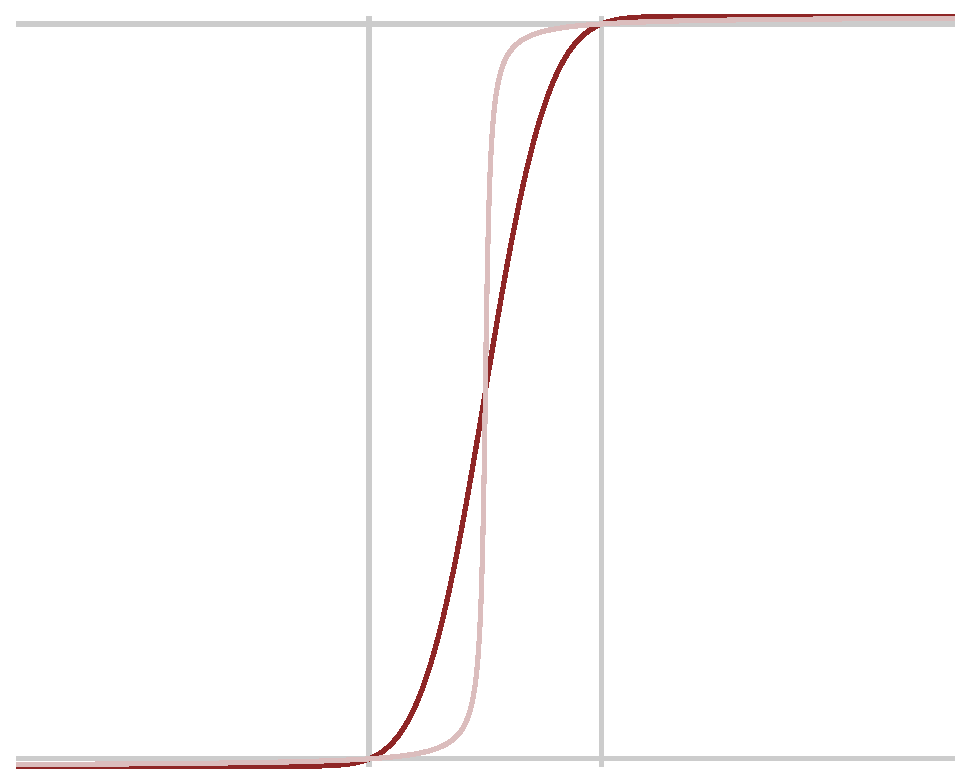
\includegraphics[height=4cm]{cdf_comp.eps}};
  \end{scope}
 
  
  \node[dark] at (-2.25, -1) { Normal };
  \node[light] at (2, -3) { Cauchy };
  
  \node[align=right] at (-2.5, 7) { Lower\\Extremity\\Threshold };
  \node[align=left] at (+2.5, 7) { Upper\\Extremity\\Threshold };
  
  \draw [->, >=stealth, line width=1] (-6.22 - 0.035, -5) -- +(12.44, 0);
  \node at (0, -6) { $\theta$ };
  
  \draw [->, >=stealth, line width=1] (-6.22, -5 - 0.035) -- +(0, 11);
  \node[rotate=90, align=center] at (-9.25, 0) { Cumulative\\Distribution Function };
  
  \node[gray80] at (-7.25, -4.9) { $0.01$ };
  \node[gray80] at (-7.25, 4.9) { $0.99$ };
  
\end{scope}

\end{tikzpicture}

\end{document}  